\chapter{Cinemática de la partícula fluida.}

\section{Repaso del operador nabla.}
En cartesianas nabla se define como:

\[\vec\nabla=\dfrac{\partial}{\partial x}\vec i + \dfrac{\partial}{\partial y}\vec j +\dfrac{\partial}{\partial z}\vec k\]

\begin{itemize}
	\item Aplicado a un campo escalar $\Phi = f(x,y,z)$
	
	\begin{itemize}
		\item Operador gradiente
		\[\vec\nabla \Phi = \left(\dfrac{\partial}{\partial x}\vec i + \dfrac{\partial}{\partial y}\vec j +\dfrac{\partial}{\partial z}\vec k\right) \Phi \text{ \textbf{(No conmutativo)}}\]

\item Laplaciano: 
\[\vec\nabla^2=\dfrac{\partial^2}{\partial x^2}+\dfrac{\partial^2}{\partial y^2}+\dfrac{\partial^2}{\partial z^2}\]

\[\vec\nabla^2\Phi=\Delta\Phi=\dfrac{\partial^2\Phi}{\partial x^2}+\dfrac{\partial^2\Phi}{\partial y^2}+\dfrac{\partial^2\Phi}{\partial z^2}\]
	\end{itemize}
	
	\item Aplicado a un campo vectorial $\vec\Phi = \phi_x(x,y,z)\vec i+\phi_y(x,y,z)\vec j+\phi_z(x,y,z)\vec z$
	\begin{itemize}
		\item Divergencia
		\[\vec\nabla \cdot \vec\Phi = \dfrac{\partial \phi_x}{\partial x} + \dfrac{\partial \phi_y}{\partial y} + \dfrac{\partial \phi_z}{\partial z}\]
		
		\item Rotacional
		
		\[
		\vec\nabla \times \vec\Phi = \begin{vmatrix}
			\vec i & \vec j & \vec k \\
			\dfrac{\partial}{\partial x} & \dfrac{\partial}{\partial y} & \dfrac{\partial}{\partial z} \\
			\phi_x & \phi_y & \phi_z \\
		\end{vmatrix}
		\]
		\item Gradiente 
		\setlength{\arraycolsep}{1.5pt}
		\renewcommand{\arraystretch}{2}
		\[\vec\nabla  \vec\Phi = \begin{bmatrix}
			\dfrac{\partial \phi_x}{\partial x} & \dfrac{\partial \phi_x}{\partial y} & \dfrac{\partial \phi_x}{\partial z} \\
			\dfrac{\partial \phi_y}{\partial x} & \dfrac{\partial \phi_y}{\partial y} & \dfrac{\partial \phi_y}{\partial z} \\
			\dfrac{\partial \phi_z}{\partial x} & \dfrac{\partial \phi_z}{\partial y} & \dfrac{\partial \phi_z}{\partial z} \\
		\end{bmatrix}\]
		
	\end{itemize}
	\item Relaciones algebraicas
	\begin{enumerate}
		\item $\vec{\nabla}(\varphi \phi) =\varphi\vec{\nabla}\phi+\phi\vec{\nabla}\varphi$
		\item $\vec{\nabla} \times \left(\vec{\nabla} \phi\right)=0$
		\item $\vec{\nabla} \cdot \left(\vec{\nabla} \times \vec{\Phi}\right) =0$
		\item $\left(\vec{\Phi}  \cdot \vec{\nabla}\right)\vec{\Phi}=\vec{\nabla} \dfrac{|\vec\Phi|}{2}^2-\vec\Phi \times \left(\vec{\Phi}  \cdot \vec{\nabla}\right) $ 
	\end{enumerate}
\end{itemize}

\section{Conceptos fundamentales.}
%\begin{figure}[H]
%	\centering
%	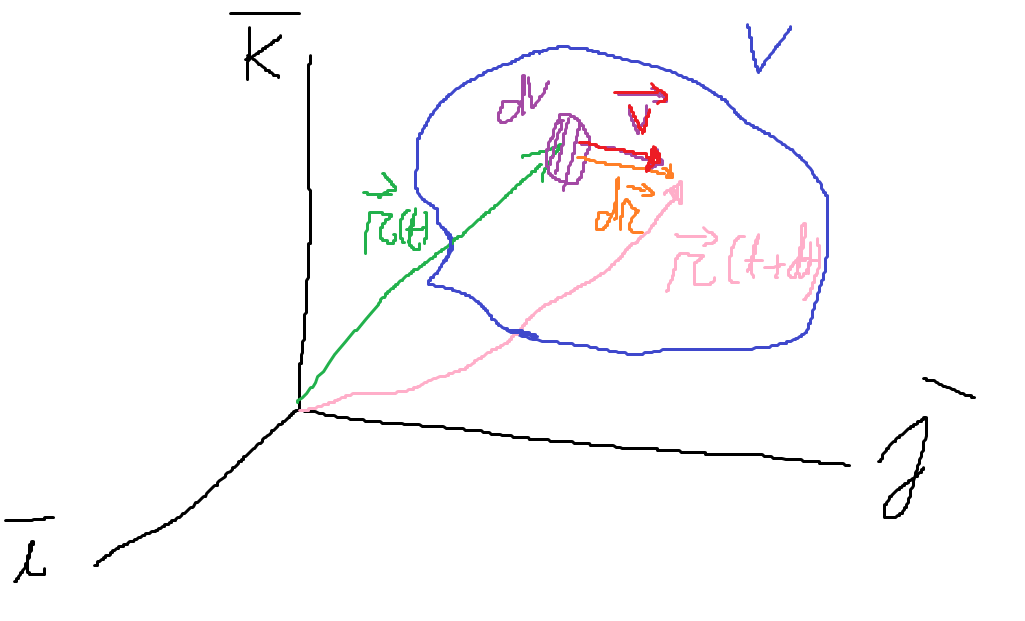
\includegraphics[width=0.5\linewidth]{imagenesTema2/magnitudesFundamentales}
%	\caption{Magnitudes fundamentales.}
%	\label{fig:magnitudesfundamentales}
%\end{figure}

\begin{figure}[H]
	\centering
		\begin{circuitikz}[scale = 0.9]
			\tikzstyle{every node}=[font=\large]
			\draw [-latex] (-2.75,17.75) -- (-2.75,22.5)node[pos=1,above]{$\vec{k}$};
			\draw [-latex] (-2.75,17.75) -- (2.5,17.75)node[pos=1,right]{$\vec{i}$};
			\draw [-latex] (-2.75,17.75) -- (-5.25,15.5)node[pos=1,left]{$\vec{j}$};
			\draw [short] (-1.5,22) .. controls (-1.25,22.75) and (-0.5,23) .. (0.5,22.75);
			\draw [short] (0.5,22.75) .. controls (1.5,22.75) and (1.75,22.75) .. (2.25,22);
			\draw [short] (2.25,22) .. controls (3.25,20.75) and (3.25,20) .. (2.25,19);
			\draw [short] (2.25,19) .. controls (1.5,18.25) and (1,18) .. (0.25,18.25);
			\draw [short] (0.25,18.25) .. controls (-1.25,19) and (-1.75,18.5) .. (-1.75,19.75);
			\draw [short] (-1.75,19.75) .. controls (-2,20.75) and (-2.25,20.5) .. (-1.5,22);
			\draw  (0,21.75) circle (0.5cm);
			\node [font=\large] at (0.25,23.25) {V};
			\node [font=\large] at (-1,21.75) {dV};
			\draw [ color={rgb,255:red,0; green,128; blue,0}, -latex] (-2.75,17.75) -- (0,21.75)node[pos=0.35,left]{$\vec{r}(t)$};
			\draw [ color={rgb,255:red,255; green,128; blue,0}, -latex] (0,21.75) -- (1.5,21.75)node[pos=1,above]{$d\vec{r}$};
			\draw [ color={rgb,255:red,255; green,0; blue,255}, -latex] (-2.75,17.75) -- (1.5,21.75)node[pos=0.35,right]{$\vec{r}(t+dt)$};
			\draw [ color={rgb,255:red,255; green,0; blue,0}, -latex] (0,21.75) -- (0.75,21.75)node[pos=1,above]{$\vec{v}$};
			\draw [short] (-0.5,21.75) .. controls (-0.25,21.5) and (0.25,21.5) .. (0.5,21.75);
			\draw [short] (-2,20.5) .. controls (-1.25,19.5) and (2.25,19.5) .. (3,20.5);
			\draw [dashed] (-2,20.5) .. controls (-1.25,21.25) and (2.25,21.25) .. (3,20.5);
			\draw [dashed] (-0.5,21.75) .. controls (-0.25,22) and (0.25,22) .. (0.5,21.75);
		\end{circuitikz}
	\caption{Magnitudes fundamentales.}
	\label{fig:magnitudesfundamentales}
\end{figure}

\begin{enumerate}
	\item \underline{\textbf{Trayectoria}}: Se determina el vector posición a partir de la velocidad. Esta ligada al enfoque lagrangiano. Tiene realidad física.
	\[\vec{v}=\dfrac{d\vec{r}}{dt} \rightarrow \vec{r}(t=0)=\vec{r_0}\]
	
	\item \underline{\textbf{Senda}}: Camino que se recorre. Es independiente del tiempo y se obtiene eliminando el tiempo t de la trayectoria. Tiene realidad física.
	
	\item \underline{\textbf{Línea de corriente}}: No tiene realidad física. Se basa den el enfoque euleriano.
	\[d\vec{r}//\vec{v}\]
	\[\vec{r}=x\vec{i}+y\vec{j}+z\vec k \rightarrow d\vec{r}=dx\vec{i}+dy\vec{j}+dz\vec{k}\]
	\[\vec{v}=v_x\vec{i}+v_y\vec{j}+v_z\vec{k}\]
	\[Si \ d\vec{r} // \vec{v} \rightarrow \vec{v} \times d\vec{r}=0= \begin{vmatrix}
		\vec i & \vec j & \vec k \\
		v_x & v_y & v_z \\
		dx & dy & dz \\
	\end{vmatrix}= \left(v_ydz-v_zdy\right)\vec{i} +\left(v_zdx-v_xdz\right)\vec{j}+\left(v_xdy-v_ydx\right) \]
	
	\[\therefore\dfrac{dz}{v_z}=\dfrac{dy}{v_y} \rightleftharpoons \dfrac{dz}{v_z}=\dfrac{dx}{v_x} \rightleftharpoons \dfrac{dx}{v_x}=\dfrac{dy}{v_y} \]
\end{enumerate}

\section{Clasificación de los flujos.}
\begin{enumerate}
	\item \underline{\textbf{Enfoque en la elección de coordenadas:}}
	\begin{enumerate}
		\item Lagrangiano: Enfoque de seguir a la partícula. 
		\[\vec{v}=\vec{v}(t(\vec{r}))=\vec{v}(t)\]
		\item Euclídeo: Enfoque de centrarse en el espacio.
		\[\vec{v}=\vec{v}(\vec{r},t)=v_x(x,y,z,t)\vec{i}+v_y(x,y,z,t)\vec{j}+v_z(x,y,z,t)\vec{k}\]
	\end{enumerate}
	\item \underline{\textbf{Dirección:}}
	\begin{enumerate}
		\item 3 direcciones ($\vec{i},\vec{j},\vec{k}$): 
		\begin{itemize}
			\item Campo vectorial tridireccional.
		\end{itemize}
		\item 2 direcciones ($\vec{i},\vec{k}$):
		\begin{itemize}
			\item Campo vectorial bidireccional.
		\end{itemize}
		\item 1 dirección ($\vec{j}$):
		\begin{itemize}
			\item Campo vectorial unidireccional.
		\end{itemize}
	\end{enumerate}
	\item \underline{\textbf{Espacio:}}
	\begin{enumerate}
		\item Si alguna componente depende de x, y, z: 
		\begin{itemize}
			\item Campo vectorial tridimensional.
		\end{itemize}
		\item Si ninguna componente depende de x, y o z: 
		\begin{itemize}
			\item Campo vectorial bidimensional.
		\end{itemize}
		\item Si todas las componentes dependen de x, y o z: 
		\begin{itemize}
			\item Campo vectorial unidimensional o monodimensional.
		\end{itemize}
		\item Si ninguna componente depende de x, y, z: 
		\begin{itemize}
			\item Campo vectorial uniforme o homogéneo.
		\end{itemize}
	\end{enumerate}
	\item \underline{\textbf{Tiempo:}}
	\begin{enumerate}
		\item Si alguna componente depende del tiempo:
		\begin{itemize}
			\item Campo vectorial no estacionario o transitorio.
		\end{itemize}
		\item Si ninguna componente depende del tiempo:
		\begin{itemize}
			\item Campo vectorial estacionario.
		\end{itemize}
	\end{enumerate}
\end{enumerate}

\section{Derivada sustancial, local y convectiva.}
Al operador diferencial de variación temporal se le denomina derivada sustancial, total o material:
\[\dfrac{D}{Dt}=\dfrac{\partial}{\partial t}+\left(\vec{v} \cdot \vec{\nabla}\right)\]

%\begin{figure}[H]
%	\centering
%	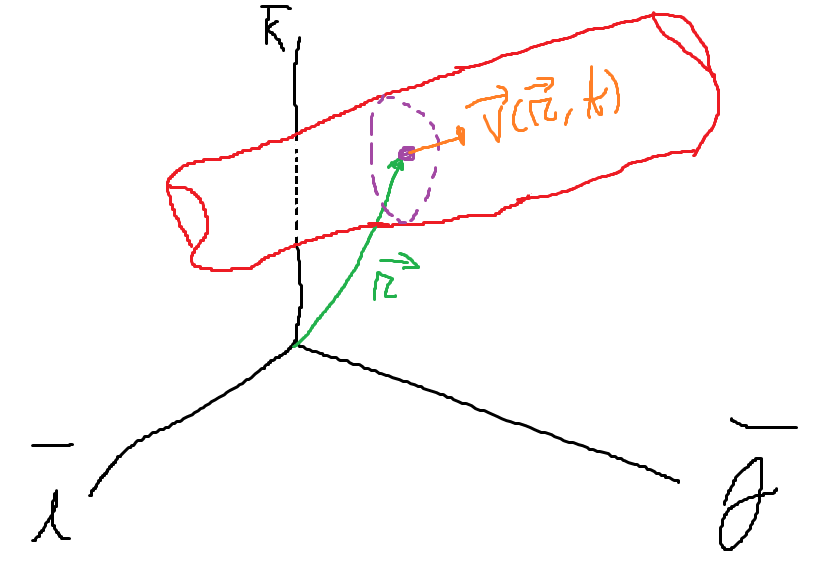
\includegraphics[width=0.5\linewidth]{imagenesTema2/derivadaSustancial}
%	\caption{Derivada sustancial.}
%	\label{fig:derivadasustancial}
%\end{figure}


\begin{figure}[!ht]
	\centering
		\begin{circuitikz}
			\tikzstyle{every node}=[font=\large]
			\draw [-latex] (-2.75,21.25) -- (-2.75,22.5)node[pos=1,above]{$\vec{k}$};
			\draw [-latex] (-2.75,17.75) -- (2.5,17.75)node[pos=1,right]{$\vec{i}$};
			\draw [-latex] (-2.75,17.75) -- (-5.25,15.5)node[pos=1,left]{$\vec{j}$};
			\draw [ color={rgb,255:red,255; green,0; blue,0}, short] (-5.25,20.75) -- (1.5,21.75);
			\draw [ color={rgb,255:red,255; green,0; blue,0}, short] (-5,18.75) -- (1.75,19.75);
			\draw [ color={rgb,255:red,255; green,0; blue,0}, short] (-5.25,20.75) .. controls (-4.75,20.25) and (-4.5,20.25) .. (-5,19.75);
			\draw [ color={rgb,255:red,255; green,0; blue,0}, short] (-5,19.75) .. controls (-5.5,19.25) and (-5.25,19) .. (-5,18.75);
			\draw [ color={rgb,255:red,255; green,0; blue,0}, short] (-5.25,20.75) .. controls (-5.5,20.5) and (-5.5,20) .. (-5,19.75);
			\draw [ color={rgb,255:red,255; green,0; blue,0}, short] (1.5,21.75) .. controls (1.75,21.25) and (1.75,21.25) .. (1.5,20.5);
			\draw [ color={rgb,255:red,255; green,0; blue,0}, short] (1.5,21.75) .. controls (1.25,21.25) and (1,21.25) .. (1.25,20.75);
			\draw [ color={rgb,255:red,255; green,0; blue,0}, short] (1.25,20.75) .. controls (1.5,20.25) and (2,20.5) .. (1.75,19.75);
			\draw [ color={rgb,255:red,255; green,0; blue,0}, dashed] (-2,21.25) .. controls (-2.5,20.5) and (-2.25,19.75) .. (-1.75,19.25);
			\draw [ color={rgb,255:red,255; green,0; blue,0}, dashed] (-2,21.25) .. controls (-1.5,20.75) and (-1.25,19.75) .. (-1.75,19.25);
			\draw [ color={rgb,255:red,0; green,128; blue,0}, -latex] (-2.75,17.75) -- (-1.75,20.25)node[pos=0.3,right]{$\vec{r}$};
			\draw [ color={rgb,255:red,0; green,128; blue,255}, -latex] (-1.75,20.25) -- (-0.25,20.5)node[pos=1,above]{$\vec{v}(\vec{r},t)$};
			\draw [dashed] (-2.75,21.25) -- (-2.75,19);
			\draw [short] (-2.75,19.25) -- (-2.75,17.75);
		\end{circuitikz}
	\caption{Derivada sustancial.}
	\label{fig:derivadasustancial}
\end{figure}

Sea $\phi=f(\vec{r},t)$ y $\vec{r}=x\vec{i}+y\vec{j}+z\vec{k}$
\[d\phi=\phi(\vec{r}+d\vec{r},t+dt)-\phi(\vec{r},t)=dx\dfrac{\partial \phi}{\partial x}+dy\dfrac{\partial \phi}{\partial y}+dz\dfrac{\partial \phi}{\partial z}+\dfrac{\partial \phi}{\partial t}dt=d\vec{r} \cdot\vec{\nabla}\phi+\dfrac{\partial \phi}{\partial t}dt\]

\[\dfrac{d\phi}{dt}=\left(\vec{v} \cdot\vec{\nabla}\right)\phi +\dfrac{\partial \phi}{\partial t} \]
\begin{itemize}
	\item Derivada convectiva: $\vec{v} \cdot\vec{\nabla}\phi$
	\item Derivada local o temporal: $\dfrac{\partial \phi}{\partial t}$
	\item Si $\phi = \vec{v}$
	\[\dfrac{d\vec{v}}{dt}=(\vec{v} \cdot\vec{\nabla})\vec{v}+\dfrac{\partial \vec v}{\partial t} \]
	\begin{itemize}
		\item Aceleración convectiva: $(\vec{v} \cdot\vec{\nabla})\vec{v}$
		\[(\vec{v} \cdot\vec{\nabla})\vec{v}=\vec{\nabla}\dfrac{|\vec{v}|}{2}^2-\vec{v} \times \left(\vec{\nabla}\times\vec{v}\right)\]
		\begin{itemize}
			\item Aceleración modular o debida a cambios del módulo de la velocidad: $\vec{\nabla}\dfrac{|\vec{v}|}{2}^2$
			\item Aceleración direccional: $-\vec{v} \times \left(\vec{\nabla}\times\vec{v}\right)$
			\begin{itemize}
				\item Vorticidad: $\vec{\omega}= \left(\vec{\nabla}\times\vec{v}\right)$
			
				\item Si la vorticidad es nula, el fluido es irrotacional y existe una función de corriente tal que:
				\[\vec{v}=-\vec{\nabla}\phi \rightarrow \vec{\nabla}\times\left(-\vec{\nabla}\phi\right)=0\]
				\item  En la literatura, a veces en lugar de hablar de vorticidad, se define velocidad de rotación como:
				\[\vec{\Omega}=\dfrac{\vec{\omega}}{2}\]
			\end{itemize}
		\end{itemize}
		\item Aceleración local: $\dfrac{\partial \vec v}{\partial t}$
	\end{itemize}
\end{itemize}
\newpage
\section{Movimiento diferencial en torno a un punto.}
A partir de la figura siguiente, se puede deducir que el movimiento diferencial es:
\[\lim_{{dt \to 0}} d\vec{v}dt=\vec{v}(\vec{r}+d\vec{r},t)dt-\vec{v}(\vec r ,t)dt\]
%\begin{figure}[H]
%	\centering
%	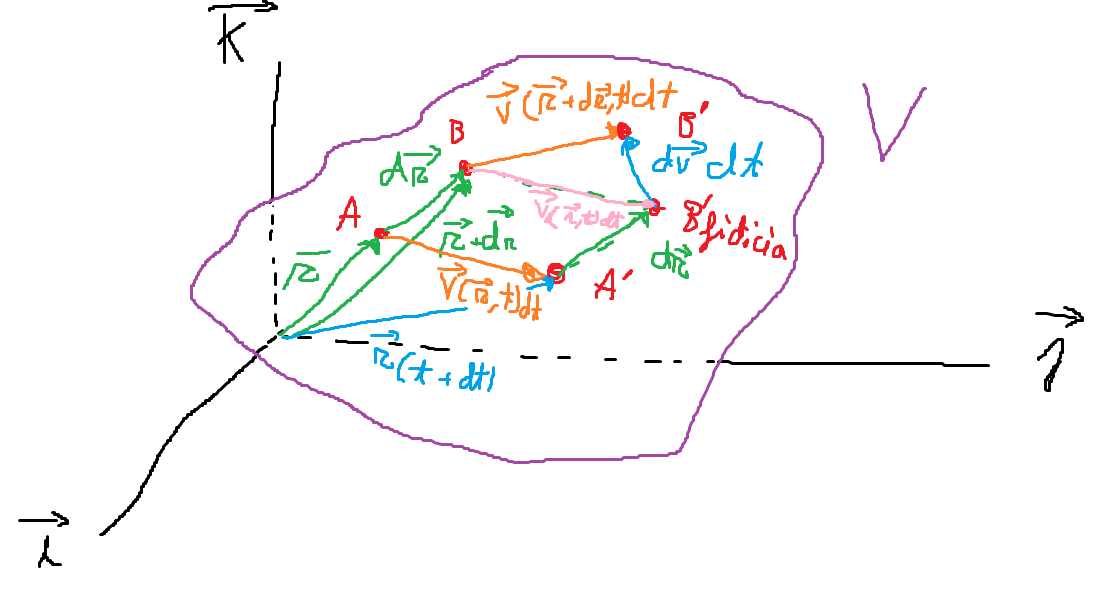
\includegraphics[width=0.7\linewidth]{imagenesTema2/movimientoDiferencial}
%	\caption{Magnitudes fundamentales del movimiento diferencial.}
%	\label{fig:movimientodiferencial}
%\end{figure}

\begin{figure}[!ht]
	\centering
		\begin{circuitikz}[scale = 1.1]
			\tikzstyle{every node}=[font=\normalsize]
			\draw [-latex] (3,17.75) -- (3.75,17.75)node[pos=1,right]{$\vec{i}$};
			\draw [-latex] (-3.25,17.25) -- (-4.25,16.25)node[pos=1,left]{$\vec{j}$};
			\draw [-latex] (-2.75,21.75) -- (-2.75,22.75)node[pos=1,above]{$\vec{k}$};
			\draw [short] (-0.5,22.25) .. controls (1.25,22.25) and (2.5,23.25) .. (3.25,22.25);
			\draw [short] (3.25,22.25) .. controls (4.25,21.25) and (3.5,21.25) .. (3.75,20);
			\draw [short] (3.75,20) .. controls (4,18.25) and (3.5,18.25) .. (2.25,17.25);
			\draw [short] (2.25,17.25) .. controls (0.75,16.25) and (0.5,17.25) .. (-1.5,17.25);
			\draw [short] (-1.5,17.25) .. controls (-3.25,17.25) and (-3.25,17) .. (-4.25,17.75);
			\draw [short] (-4.25,17.75) .. controls (-5,18.75) and (-4.75,19.5) .. (-3.75,20.75);
			\draw [short] (-3.75,20.75) .. controls (-3,21.75) and (-2.5,22) .. (-0.5,22.25);
			\node [font=\large] at (0.75,22.75) {V};
			\draw [ color={rgb,255:red,0; green,128; blue,0}, -latex] (-2.75,17.75) -- (-2,19.75)node[pos=0.9,left]{$\vec{r}$};
			\draw [ color={rgb,255:red,0; green,255; blue,0}, -latex] (-2,19.75) -- (-1,20)node[pos=0.5,sloped,above]{$d\vec{r}$};
			\draw [ color={rgb,255:red,0; green,176; blue,0}, -latex] (-2.75,17.75) -- (-1,20)node[pos=0.6,above,sloped]{$\vec{r}+d\vec{r}$};
			\draw [ color={rgb,255:red,255; green,128; blue,0}, -latex] (-2,19.75) -- (0.5,19.25)node[pos=0.5,below,sloped]{$\vec{v}(\vec{r},t)dt$};
			\draw [ color={rgb,255:red,0; green,128; blue,255}, -latex] (-2.75,17.75) -- (0.5,19.25)node[pos=0.75,below,sloped]{$\vec{r}(t+dt)$};
			\draw [ color={rgb,255:red,0; green,255; blue,0}, -latex] (0.5,19.25) -- (1.5,19.5)node[pos=0.5,below,sloped]{$d\vec{r}$};
			\draw [ color={rgb,255:red,255; green,0; blue,255}, -latex] (-1,20) -- (1.5,19.5)node[pos=0.55,above,sloped]{$\vec{v}(\vec{r},t)dt$};
			\draw [ color={rgb,255:red,0; green,128; blue,255}, -latex] (1.5,19.5) -- (1,21.25)node[pos=0.5,above,sloped]{$d\vec{v}dt$};
			\draw [ color={rgb,255:red,255; green,128; blue,0}, -latex] (-1,20) -- (1,21.25)node[pos=0.65,above,sloped]{$\vec{v}(\vec{r}+d\vec{r},t)dt$};
			\draw [dashed] (-2.75,21.75) -- (-2.75,17.75);
			\draw [dashed] (-3.25,17.25) -- (-2.75,17.75);
			\draw [dashed] (-2.75,17.75) -- (3,17.75);
		\end{circuitikz}
	\caption{Magnitudes fundamentales del movimiento diferencial.}
	\label{fig:movimientodiferencial}
\end{figure}

Operando y despreciando el diferencial de tiempo:
\[d\vec{v}=\vec{v}(\vec{r}+d\vec{r},t)-\vec{v}(\vec r ,t)=d\vec{r}\cdot(\vec{\nabla}\vec{v})\]
Donde $\vec{\nabla}\vec{v}$ es el tensor gradiente de la velocidad:
\setlength{\arraycolsep}{1.5pt}
\renewcommand{\arraystretch}{2}
\[\vec{\nabla}\vec{v}=\begin{bmatrix}
	\dfrac{\partial v_x}{\partial x} & \dfrac{\partial v_x}{\partial y} & \dfrac{\partial v_x}{\partial z} \\
	\dfrac{\partial v_y}{\partial x} & \dfrac{\partial v_y}{\partial y} & \dfrac{\partial v_y}{\partial z} \\
	\dfrac{\partial v_z}{\partial x} & \dfrac{\partial v_z}{\partial y} & \dfrac{\partial v_z}{\partial z} \\
\end{bmatrix}=\dfrac{1}{2}\left[\vec{\nabla}\vec{v}+\left(\vec{\nabla}\vec{v}\right)^t\right]+\dfrac{1}{2}\left[\vec{\nabla}\vec{v}-\left(\vec{\nabla}\vec{v}\right)^t\right]=\overline{\overline{\xi}}+\overline{\overline{\gamma}}\]
Las variables que aparecen, son $\overline{\overline{\xi}}$ el tensor de velocidad de deformación (simétrico) y $\overline{\overline{\gamma}}$ el tensor de velocidad de rotación.
\newpage
\setlength{\arraycolsep}{1.5pt}
\renewcommand{\arraystretch}{2}
\[\overline{\overline{\xi}}=\begin{bmatrix}
	\dfrac{\partial v_x}{\partial x} & \dfrac{1}{2}\left(\dfrac{\partial v_x}{\partial y}+\dfrac{\partial v_y}{\partial x}\right) & \dfrac{1}{2}\left(\dfrac{\partial v_x}{\partial z}+\dfrac{\partial v_z}{\partial x}\right) \\
	\dfrac{1}{2}\left(\dfrac{\partial v_x}{\partial y}+\dfrac{\partial v_y}{\partial x}\right) & \dfrac{\partial v_y}{\partial y} & \dfrac{1}{2}\left(\dfrac{\partial v_y}{\partial z} +\dfrac{\partial v_z}{\partial y}\right) \\
	\dfrac{1}{2}\left(\dfrac{\partial v_x}{\partial z}+\dfrac{\partial v_z}{\partial x}\right) & \dfrac{1}{2}\left(\dfrac{\partial v_y}{\partial z} +\dfrac{\partial v_z}{\partial y}\right) & \dfrac{\partial v_z}{\partial z} \\
\end{bmatrix}\]
\setlength{\arraycolsep}{1.5pt}
\renewcommand{\arraystretch}{2}
\[\overline{\overline{\gamma}}=\begin{bmatrix}
0 & \dfrac{1}{2}\left(\dfrac{\partial v_x}{\partial y}-\dfrac{\partial v_y}{\partial x}\right) & \dfrac{1}{2}\left(\dfrac{\partial v_x}{\partial z}-\dfrac{\partial v_z}{\partial x}\right) \\

	-\dfrac{1}{2}\left(\dfrac{\partial v_x}{\partial y}-\dfrac{\partial v_y}{\partial x}\right) & 0 & \dfrac{1}{2}\left(\dfrac{\partial v_y}{\partial z} -\dfrac{\partial v_z}{\partial y}\right) \\
	
	-\dfrac{1}{2}\left(\dfrac{\partial v_x}{\partial z}-\dfrac{\partial v_z}{\partial x}\right) & -\dfrac{1}{2}\left(\dfrac{\partial v_y}{\partial z} -\dfrac{\partial v_z}{\partial y}\right) & 0 \\
\end{bmatrix}\]
Por tanto, aplicado al movimiento:
\[d\vec{v}=d\vec{r}\cdot(\vec{\nabla}\vec{v})=d\vec{r}\cdot\overline{\overline{\xi}}+d\vec{r}\cdot\overline{\overline{\gamma}}\]
Donde:
\begin{itemize}
	\item Movimiento velocidad de deformación: $d\vec{r}\cdot\overline{\overline{\xi}}$ que representa las deformaciones lineales (diagonal) y angulares (fuera de la diagonal).
	\begin{itemize}
		\item Si la traza de $\overline{\overline{\xi}}$ es nula, el fluido es incompresible y, por tanto de densidad constante.
	\end{itemize}
	\item Movimiento velocidad de rotación: $\overline{\overline{\gamma}}$ que representa el movimiento del fluido como si fuera un sólido rígido.
	\begin{itemize}
		\item Se puede relacionar este tensor con la vorticidad y se demuestra que:
		\[\overline{\overline{\gamma}} =\dfrac{1}{2}\vec{\omega}\times d \vec{r}=\left(\vec{\nabla}\times\vec{v}\right)\times d \vec{r}=\begin{bmatrix}
			0 & -\dfrac{1}{2}\omega_z & \dfrac{1}{2}\omega_y \\
			\dfrac{1}{2}\omega_z & 0 & -\dfrac{1}{2}\omega_x\\	
			-\dfrac{1}{2}\omega_y & \dfrac{1}{2}\omega_x & 0 \\
		\end{bmatrix}\]
	\end{itemize}
\end{itemize}
\section{Movimiento de la partícula fluida en una dirección.}
Se parte de la expresión deducida anteriormente pero expresando el $d\vec{r}$ mediante módulo dirección, esta expresión, también se suele denominar movimiento vectorial:
\[d\vec{v}=d\vec{r}\cdot\left(\vec{\nabla}\vec{v}\right)=d\vec{r}\cdot\left(\overline{\overline{\xi}}+\overline{\overline{\gamma}}\right)=|d\vec{r}|\vec{n}\cdot\left(\overline{\overline{\xi}}+\overline{\overline{\gamma}}\right)\]
%\begin{figure}[H]
%	\centering
%	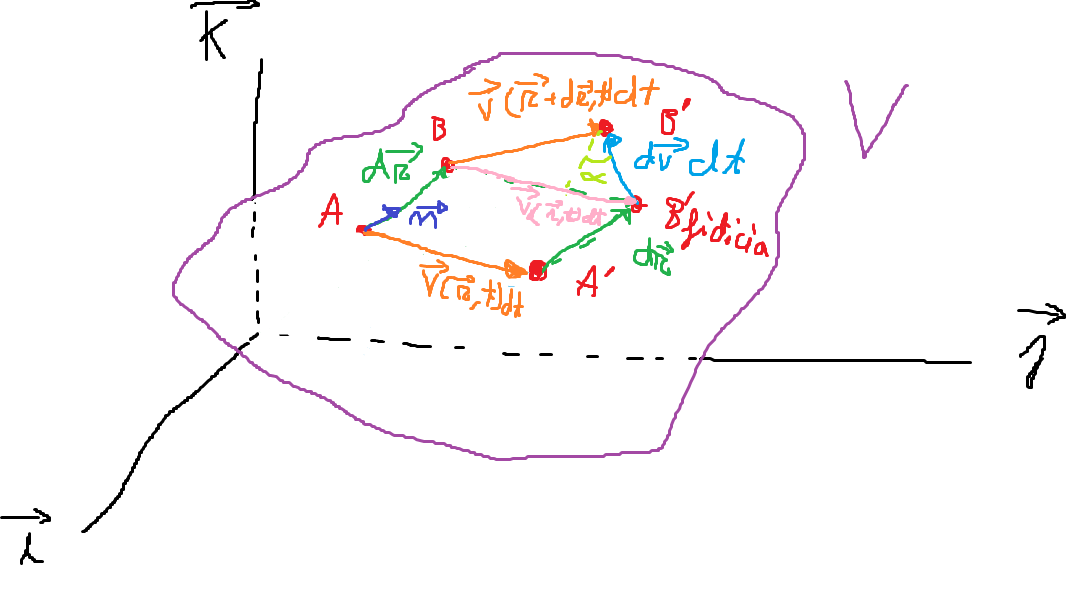
\includegraphics[width=0.7\linewidth]{imagenesTema2/movimientoDireccion}
%	\caption{Magnitudes fundamentales del movimiento de la partícula fluida.}
%	\label{fig:movimientodireccion}
%\end{figure}

\begin{figure}[H]
	\centering
		\begin{circuitikz}
			\tikzstyle{every node}=[font=\large]
			\draw [-latex] (-1.75,15.75) -- (-1.75,21.25)node[pos=1,above]{$\vec{k}$};
			\draw [-latex] (3.75,15.75) -- (5.75,15.75)node[pos=1,right]{$\vec{i}$};
			\draw [-latex] (-1.75,15.75) -- (-3.25,14.25)node[pos=1,left]{$\vec{j}$};
			\draw [ color={rgb,255:red,128; green,0; blue,255}, short] (-1.25,20) .. controls (-2,21.5) and (-0.25,20.75) .. (1.5,21.5);
			\draw [ color={rgb,255:red,128; green,0; blue,255}, short] (1.5,21.5) .. controls (3.25,21.75) and (3.25,21) .. (5,20.5);
			\draw [ color={rgb,255:red,128; green,0; blue,255}, short] (5,20.5) .. controls (5.75,20.25) and (5.25,19.5) .. (5.5,18.25);
			\draw [ color={rgb,255:red,128; green,0; blue,255}, short] (5.5,18.25) .. controls (5.75,16.75) and (5,17.25) .. (4.25,16.25);
			\draw [ color={rgb,255:red,128; green,0; blue,255}, short] (4.25,16.25) .. controls (3,14.75) and (2,16.25) .. (-0.25,16);
			\draw [ color={rgb,255:red,128; green,0; blue,255}, short] (-0.25,16) .. controls (-1.5,16.25) and (-1.75,17) .. (-1.5,18);
			\draw [ color={rgb,255:red,128; green,0; blue,255}, short] (-1.5,18) .. controls (-1.25,19) and (-0.75,19) .. (-1.25,20);
			\node [font=\large, color={rgb,255:red,128; green,0; blue,255}] at (4.25,21.25) {V};
			\draw [ color={rgb,255:red,128; green,0; blue,255}, -latex] (-0.5,17.75) -- (0.25,18.75)node[pos=0.5,left]{$\vec{n}$};
			\draw [ color={rgb,255:red,0; green,128; blue,0}, -latex] (-0.5,17.75) -- (1,19.75)node[pos=0.8,left]{$d\vec{r}$};
			\draw [ color={rgb,255:red,255; green,128; blue,0}, -latex] (1,19.75) -- (3.5,20.75)node[pos=0.5,sloped,above]{$\vec{v}(\vec{r}+d\vec{r},t)dt$};
			\draw [ color={rgb,255:red,0; green,128; blue,255}, -latex] (4.25,19.25) -- (3.5,20.75)node[pos=0.5,right]{$d\vec{v}dt$};
			\draw [ color={rgb,255:red,255; green,128; blue,0}, -latex] (-0.5,17.75) -- (2.75,17)node[pos=0.5,sloped,above]{$\vec{v}(\vec{r},t)dt$};
			\draw [ color={rgb,255:red,0; green,128; blue,0}, -latex] (2.75,17) -- (4.25,19.25)node[pos=0.5,left]{$d\vec{r}$};
			\draw [ color={rgb,255:red,255; green,128; blue,255}, -latex] (1,19.75) -- (4.25,19.25)node[pos=0.5,sloped,below]{$\vec{v}(\vec{r},t)dt$};
			\draw [ color={rgb,255:red,0; green,128; blue,0}, dashed] (3.5,20.75) -- (2.75,19.5);
			\draw [ color={rgb,255:red,0; green,128; blue,0}, short] (3,20) .. controls (3.25,19.75) and (3.75,19.75) .. (4,19.75)node[pos=0.45,above]{$\alpha$};
			\draw [dashed] (3.75,15.75) -- (1.75,15.75);
			\draw [short] (1.75,15.75) -- (-1.75,15.75);
		\end{circuitikz}
	\caption{Magnitudes fundamentales del movimiento de la partícula fluida.}
	\label{fig:movimientodireccion}
\end{figure}

Si se aplica a una dirección concreta, también suele denominarse como movimiento escalar:
\[d\vec{v}\cdot\vec{n}=d\vec{r}\cdot\left(\vec{\nabla}\vec{v}\right)=d\vec{r}\cdot\left(\overline{\overline{\xi}}+\overline{\overline{\gamma}}\right)=|d\vec{r}|\vec{n}\cdot\left(\overline{\overline{\xi}}+\overline{\overline{\gamma}}\right)\cdot\vec{n}=\vec{n}\cdot\left(\overline{\overline{\xi}}+\overline{\overline{\gamma}}\right)\cdot\vec{n}\]
Como la dirección no es más que una composición de las distintas direcciones, se puede dividir por coordenadas:
\begin{itemize}
	\item Los términos de deformación:
	\begin{itemize}
		\item Si $\vec{n}=\vec{i}\rightarrow\vec{i}\cdot\overline{\overline{\xi}}\cdot\vec{i}=\xi_{11}$
		\item Si $\vec{n}=\vec{j}\rightarrow\vec{j}\cdot\overline{\overline{\xi}}\cdot\vec{j}=\xi_{22}$
		\item Si $\vec{n}=\vec{k}\rightarrow\vec{k}\cdot\overline{\overline{\xi}}\cdot\vec{k}=\xi_{33}$
	\end{itemize}
	\item Los términos de velocidad de rotación:
	\begin{itemize}
		\item Para todo vector $\vec{n}\cdot\overline{\overline{\gamma}}\cdot\vec{n}=0$
	\end{itemize}
\end{itemize}

